\begin{figure}[H]
    \centering
    \caption{Covering the points with $f(x) = 1$}
    \label{fig::sin-explanation}
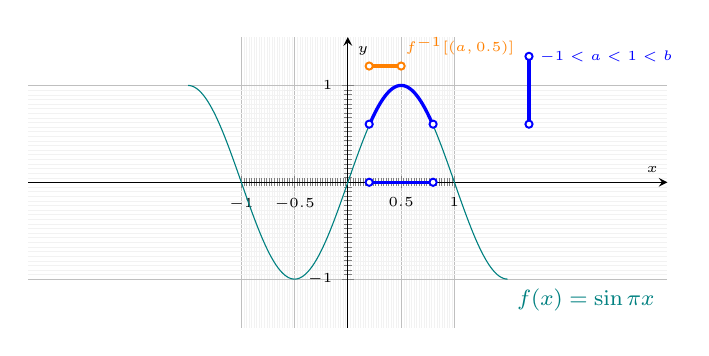
\begin{tikzpicture}
    \begin{axis}[
        width = 0.8\textwidth,
        grid=both,
        minor tick num=20,
        grid style={line width=.1pt, draw=gray!10},
        major grid style={line width=.1pt,draw=gray!50},
        axis lines=middle,clip=false,
        height = 150,
        xmin=-3,xmax=3,ymin=-1.5,ymax=1.5,
        ytick={-1,0,1},
        xtick={-1,-0.5,0,0.5,1},
        font=\tiny,
        xticklabels={$-1$,$-0.5$,$0$,$0.5$,$1$},
        xticklabel style={black},
        xlabel=$x$,
        ylabel=$y$
    ]
    \draw[very thick, blue] (axis cs:1.7,0.6) -- (axis cs:1.7,1.3) node[right, font=\tiny] {$-1<a<1<b$};
    \fill [color=white,draw=blue,line width=0.7pt] (axis cs:1.7,0.6) circle (1.3pt);
    \fill [color=white,draw=blue,line width=0.7pt] (axis cs:1.7,1.3) circle (1.3pt);

    \addplot[domain=-1.5:1.5,samples=150,teal]{sin(deg(pi*x))}
                                node[below right,pos=1,font=\footnotesize]{$f(x)=\sin \pi x$};

    \addplot[domain=.2:0.8,samples=100, very thick,blue]
        {sin(deg(pi*x))} node[below right,pos=1,font=\footnotesize]{};
    \addplot[domain=.2:0.8,samples=100, very thick,blue]
        {0} node[below right,pos=1,font=\footnotesize]{};

    \fill [color=white,draw=blue,line width=0.7pt] (axis cs:0.2,0.6) circle (1.3pt);
    \fill [color=white,draw=blue,line width=0.7pt] (axis cs:0.8,0.6) circle (1.3pt);

    \fill [color=white,draw=blue,line width=0.7pt] (axis cs:0.2,0) circle (1.3pt);
    \fill [color=white,draw=blue,line width=0.7pt] (axis cs:0.8,0) circle (1.3pt);
    
    \addplot[domain=.2:0.5,samples=100, very thick, orange]
        {1.2} node[above right,pos=0.8,font=\tiny]{$f^{-1}[(a,0.5)]$};
    \fill [color=white,draw=orange,line width=0.7pt] (axis cs:0.2,1.2) circle (1.3pt);
    \fill [color=white,draw=orange,line width=0.7pt] (axis cs:0.5,1.2) circle (1.3pt);
    \end{axis}
  \end{tikzpicture}
\end{figure}
